\documentclass[11pt,a4paper]{article}
\usepackage[hyperref]{acl2020}
\usepackage{times}
\usepackage{tabularx}
\usepackage{latexsym}
\usepackage{graphicx}
\usepackage{subfig}
\usepackage{commath}
\renewcommand{\UrlFont}{\ttfamily\small}
\newcommand{\spacemanidol}[1]{\textcolor{orange}{\bf \small [#1 --dc]}}
\newcommand{\hayley}[1]{\textcolor{pink}{\bf \small [#1 --h]}}
\setlength\titlebox{5cm}
\newcommand\BibTeX{B\textsc{ib}\TeX}
\usepackage{microtype}
\aclfinalcopy 
\title{LING 573: Document Summarization Project Report}
\author{Daniel Campos, Sicong Huang, Shunjie Wang, Simola Nayak, \and Hayley Luke \\ University of Washington \\ {\tt\{dacamp, huangs33, shunjiew, simnayak, jhluke\}@uw.edu}}
\begin{document}
\maketitle
\begin{abstract}
We design and implement Mockingbird, a topic-focused multi-document extractive summarization system. Building on the LexRank graph algorithm our system uses sentence similarity and topic-sentence bias to produce candidates. Next, the ranked sentences are selected to limit redundancy and stay under 100 words. Our system outperforms the LEAD and MEAD baseline by a fair margin. Future work will focus on forms of text representation and processing along with more complex selection and sorting can improve system performance
\end{abstract}
\section{Introduction}
Topic oriented document clusters like AQUAINT \cite{Graff2002TheAC} and ACQUAINT-2 have been used as a starting point to explore various methods for document summarization. More specifically, these corpora have been used to study extractive multi-document topic summarization. These corpora have been the focus of study in TAC(Text Analytics Conference) \cite{Dang2008OverviewOT} summarization shared task. In the formalization of this task give a topic and a set of news wire documents a competitive system should create a high quality summary of the topic using sentences from the documents. Systems are expected to produce summaries up to 100 words and summaries should be coherent and not contain duplication. Once summaries are generated for all the topics being studied, methods are evaluated and compared using the standard ROUGE metric \cite{Lin2004ROUGEAP}.

Our exploratory system, called Mockingbird (MB), is based on the Biased LexRank graph approach \cite{Otterbacher2009BiasedLP}. In this approach, we provide a ranking of all candidate sentences by combining a matrix which represents sentence similarity with a topic and sentence similarity. After a ranking is produced sentences are selected to maximize their LexRank score but minimize duplication of content. Our method relies on word vectors \cite{Mikolov2013DistributedRO} from the spaCy library \footnote{https://spacy.io/} to represent sentences and we experiment with the effects of evaluating complete sentences, sentences without stop words, and only the nouns in the sentences. After we have a set of candidate sentences we sort them in reverse chronological order and then realize the content to match the TAC output format. To understand our system performance we compare our systems ROUGE-1 and ROUGE-2 scores when compared to LEAD, and MEAD baselines. Our system across the board performs favorably as we beat the two baselines(MEAD and LEAD). However, our system lags behind the top system from TAC 2010 by a significant margin.
\section{System Overview}
Mockingbird has been designed as a simple end-to-end pipeline with the goal of producing a structure we can continue to tweak and modify to understand the effect of various changes have on downstream performance. The pipeline, represented in Figure \ref{fig:overview}, broadly has 4 steps: document input and processing, content selection, information ordering, content realization.
\begin{figure}[h]
  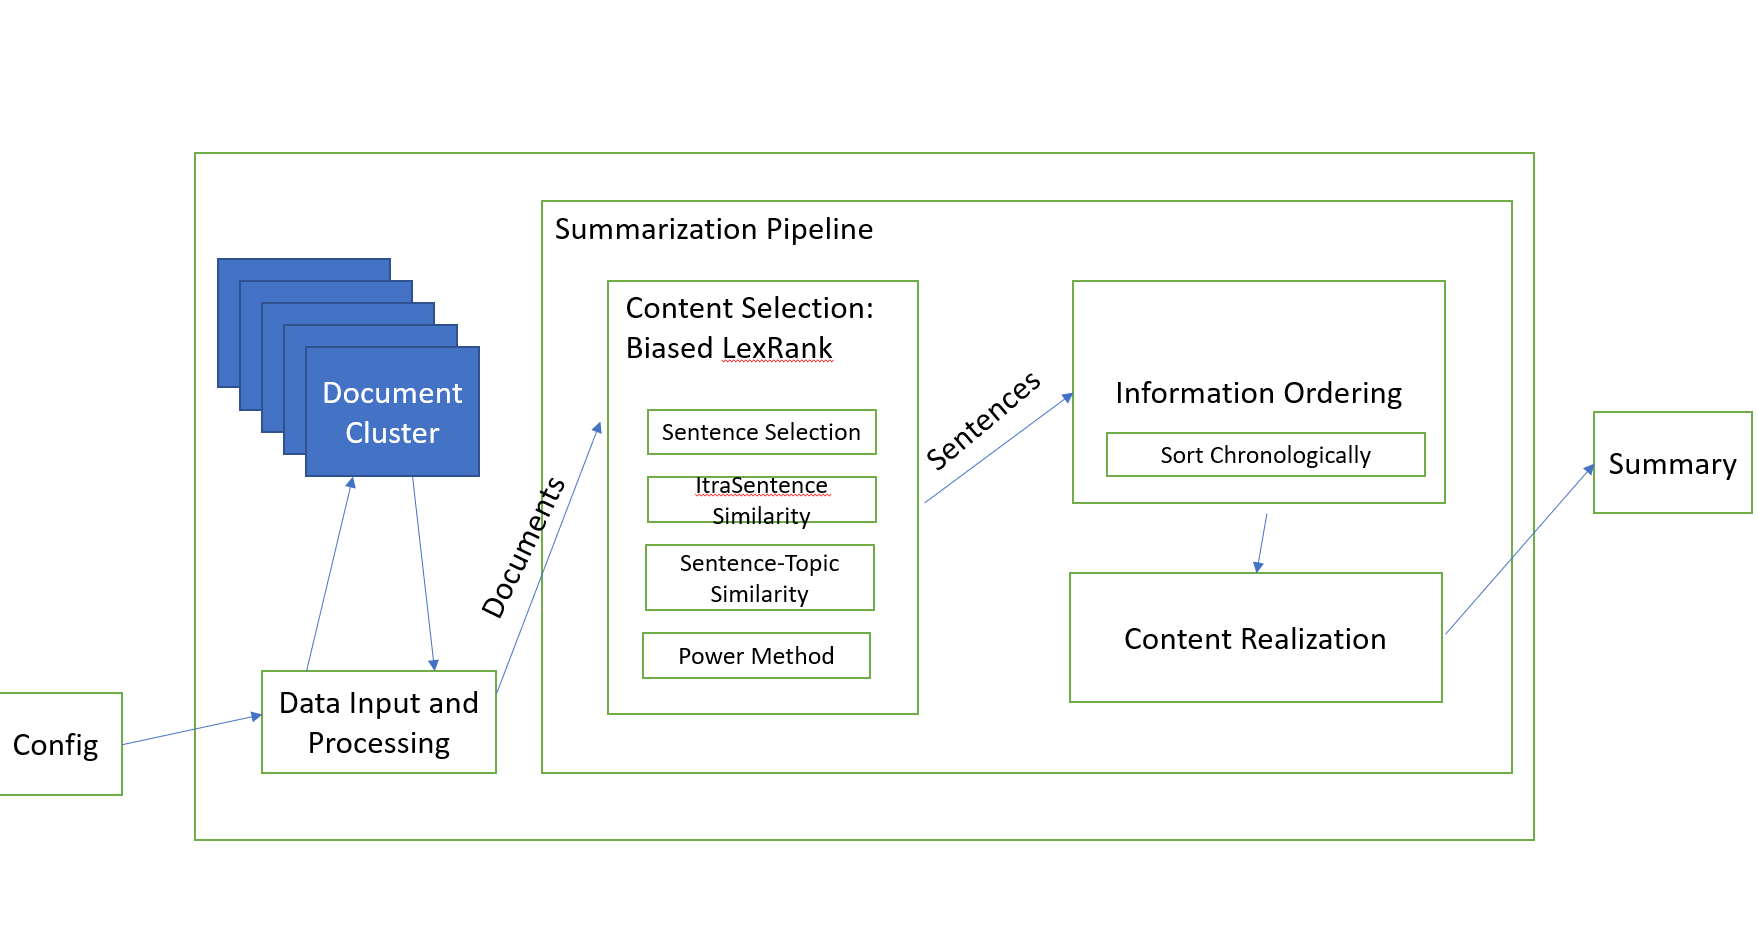
\includegraphics[width=\linewidth]{doc/overview.png}
  \caption{Overview Of Mockingbird's Architecture}
  \label{fig:overview}
\end{figure}
\section{Approach}
In this section we will describe the in detail each of the steps our system takes to summarize topics.
\subsection{Data Input and Processing}
Documents come from the ACQUAINT and ACQUAINT-2 corpus and are a mixture of HTML and XML. The document pipeline takes as an input a configuration file (XML) which details a series of topics and associates the them with a group of document ID's. Using this configuration file, we compile a list of topics, and use the document ID's to determine the path to the relevant corpus file on disk. We then search the file for the information relevant to our specific document ID, and extract the text, the date, and the title. We clean the data, converting the date to a usable format, stripping excess white space and symbols in the text, and normalizing quotation marks. We then break the text into sentences using spaCy's sentence tokenization, and remove sentences that appear to be questions or bylines.
\subsection{Content Selection}
Next, there is the content selection pipeline. In this step we consume the structured information from the processing pipeline and produce a candidate set of sentences. Our system selects content using a modified version of the Biased LexRank Graph approach. This method computes a intrasentence and topic-sentence similarity which is used to create a similarity matrix and a bias vector. In this method, each node of the graph represents a sentence and edges between nodes are represented by their intrasentence similarity. This representation allows ranking of sentences to be based on their similarity to the topic and their centrality in the topic document clustering. Our method differs from the original implementation of Lex
Rank \cite{otterbacher-etal-2005-using} as we leverage word embeddings instead of their tf-idf implementation.

For each topic we first assemble all sentences in scope of the topic that have at least 4 words. Then, for each sentence, we create a sentence representation. We explore using average word embeddings, IDF-weighted word embeddings, and transformer based sentence embeddings \cite{reimers-2019-sentence-bert}. For our sentence representations we use spaCy to create a vector representation for each word in the sentence. Then we average all the embeddings in the sentence to produce a de-facto sentence embedding. We explore using this method to create word representations where we drop stop words, nouns only, and use the whole sentence. This method leverages the word embeddings known as GloVe \cite{Pennington2014GloveGV} for word embeddings. IDF-weighted word embedding uses the same GloVe embedding; however, instead of averaging across all words, we take the weighted average using each word's IDF value as weight. For our transformer based sentence embedding we use a Sentence-BERT which relies on a Siamese sentence representation fine tuned model. Using these representations, we follow equation \ref{equation:1} to we generate a two dimension matrix representing the cosine similarity between all the sentences related to the topic. Additionally, we create a bias 1d vector which represents the cosine similarity between the topic and each sentence. For inter-sentential cosine similarity, we use a minimum threshold of 0.3 as we find word similarity tends to be higher then tf-idf similarity.

We now use sentence embeddings based on \cite{reimers-2019-sentence-bert}
\begin{equation}
\label{equation:1}
similarity(u,v) = cos(u,v) = \frac{u * v}{\norm{u}\norm{v}}
\end{equation}
Using the bias vector and the inter sentence similarity matrix we compute a LexRank for each sentence using the equation \ref{equation:2} where $s$ is a sentence, $q$ is the topic string, $d$ is the weight bias for the topic(set to 0.8), and $S$ represents all sentence in the topic. 
\begin{equation}
   bias(s|q_ =  \frac{cos(s,q)}{\sum_{a \in S} cos(a,q) }
\end{equation}
\begin{equation}
    sentsim(s,S) = \sum_{s_1 \in S} \frac{cos(s,s_1)}{\sum_{s_2 \in S} cos(s_1,s_2) }
\end{equation}
\begin{equation}
\label{equation:2}
lr(s|q) = d * bias(s|q) + (1-d) * sentsim(s,S)
\end{equation}

In our system, we turn our 2d inter-sentential similarity matrix ($IS$) and bias vector ($BV$) into a matrix $M$ using equation \ref{equation:3}.  Then, we implement the power method, as described in equation \ref{equation:4}, to produce a converged LexRank values for each sentence. As LexRank represents sentence probabilities we initial have a uniform distribution (all sentences are equally likely to show up) and we use the power method until the method converges or an $\epsilon$ of 0.3.
\begin{equation}
\label{equation:3}
M = [d * IS + (1-d) * BV]^T
\end{equation}
\begin{equation}
\label{equation:4}
P_t = M * p_t-1
\end{equation}

Once we have assembled sampling probabilities for each sentence we select sentences until we have either used all candidate sentences or reached the target length of 100 words. Sentences are initially ranked by LexRank score and we select candidates that have less than a 0.6 cosine similarity to all other selected sentence. This filter is applied to minimize sentence redundancy. 
\subsection{Information Ordering}
Following content selection we run our information ordering system. The method used is based on the entity grid approach proposed in \citet{barzilay-lapata-2008-modeling}. In order to build an entity grid for a document, we first use spaCy pre-trained models to perform POS tagging and dependency parsing on the sentences, in order to identify all the nouns and label them accordingly as $S, O, X$ according to their dependency tags. Each column in the grid represents one noun, and each row represents one sentence. The cells are the labels above indicating the dependency tag of the noun in the sentence.

We then vectorize each entity grid to a feature vector. The features are bigram transitions in $\{S,O,X,-\}^2$. Thus, there are 16 features in total. A transition is defined as how symbols in each column change from one to another in adjacent sentence rows. The value for each feature is the probability of the particular bigram transition occurring among all transitions.

We treat sentence ordering as a ranking problem, and our goal is to learn a ranking function such that given a set of candidate sentence orderings, the function ranks the candidates and the best is kept as the optimal sentence ordering. We train an SVM model for this purpose using $SVM^{rank}$ \citep{joachims2006training}. The training data used is sampled from TAC 2009 human-created model summaries. We randomly chose 80 documents in the set and build entity grids and feature vectors for them. Then, for each of the 80 documents, we generate up to 20 random sentence permutations of the document and their corresponding feature vectors. We pair each random permutation with the gold ordering, which is up to 1600 pairs in total, and we label gold sentence with a higher rank than the random permutation, so the model should favor the gold sentence which is more coherent.

Once the ranking model is trained, we can use it for predicting rank of new instances. Given selected sentences from the content selection component, we generate a number of sentence permutations as candidate orderings. One of the candidate is the chronologically ordered sentence. We then build entity grid and feature vectors for all candidates, and predict the rankings of the candidates and keep the best according to our SVM ranking model's prediction. 
\subsection{Content Realization}
Following information ordering we run our content realization system. In addition to cleaning with regular expressions, largely as a redundancy for the cleanup done during preprocessing. For this deliverable, two naive techniques to improve readability were attempted but proved to add computational overhead and worsened ROUGE-2: splitting large sentences in half and trimming gratuitous nodes from the resulting sentences. As a result, we had to revert to the previous iteration of our content realization system.
\subsubsection{Attempted Improvement}
A three-stage pipeline was introduced: cleanup followed by splitting sentences followed by trimming gratuitous modifiers. Splitting the large sentences, consisting of anything larger than 7 or 8 tokens, was a largely naive procedure applied strictly to sentences that contained multiple nodes labeled as "ROOT" in the parse. The procedure found the first node labeled as 'cc' by the SpaCy parse and split the sentence at that index creating two new sentences. The impact of such an approach included contrast discourse relations (e.g. those from the conjunction but) potentially being lost. An example of the result of such a split is as follows, with changed areas underlined:\\

\begin{tabular}{l p{55mm}}
\textbf{Original} & Next week the Security Council is to review the sanctions imposed against Baghdad following the invasion of \underline{Kuwait, and western} diplomats are predicting that the four-year-old embargo will remain in force.\\
\textbf{Split} & Next week the Security Council is to review the sanctions imposed against Baghdad following the invasion of \underline{Kuwait. Western} diplomats are predicting that the four-year-old embargo will remain in force.
\end{tabular}\\ \\ \\ \\
Similarly, long sentences extracted from newspapers were also split at semicolons. Both approaches to splitting long sentences improved individual sentence readability- as determined by humans; however, the small sentences led to discourse simplified beyond the degree typical of such a summary.\\ \\
After splitting sentences, the SpaCy parser was reused in order to parse the split sentences for modifier removal. This step removed both adjectives and adverbs alike. Because of the naive nature of such deletions, informative modifiers were removed in addition to gratuitous ones, reducing readability. Such deletions meant sentences with degree modifiers ended up with less information, and this was particularly problematic for phrases like "high risk" and "low probability." Due to such word deletions, ROUGE-1 and ROUGE-2 recall scores dropped significantly; conversely, the conciseness-motivated revisions meant ROUGE-1 precision increased.
\subsection{Evaluation}
We use both automatic (ROUGE) and human evaluation to assess our system performance. 

To run the ROUGE evaluation script, we generate a configuration file that associates our system's output summaries and the provided gold standard human summaries. For easy comparison, we only consider the recall scores of ROUGE-1 and ROUGE-2. 

A human evaluation on readability is performed on a subset of the output of the final iteration of our system. Each annotator is asked to assign a score between 1 to 5 to a system summary. Criteria is as follows:
\vspace{-0.2cm}
\begin{enumerate}
\itemsep -0.1cm
    \item  poor: confusing, bizarre, or incoherent; unrecoverable contexts
    \item fair: several readability problems, but most are recoverable
    \item ok: mostly understandable; a few minor readability or flow issues
    \item good: fully coherent; minor stylistic problems
    \item excellent: idiomatically correct, readable, and cohesive
\end{enumerate}
\section{Results}
To evaluate our system performance we ran our system on the 2010 TAC shared evaluation task. The 2010 TAC task has 43 systems including baselines. The 1st baseline (LEAD), created summaries using the first 100 words from the most recent document. The 2nd baseline was the output of the MEAD summarization system \cite{Radev2003MEADRM}. We have also included system 43 and system 22 as benchmarks because they had the best performance in the shared task(eval and dev set respectively). We evaluate models according to their ROUGE-2 and ROUGE-1 Recall scores on the devtest portion of the 2010 TAC task. Our system has variants that explore using stop words removal for word vectors (NS), IDF, and a transformer model. Each implementation includes the two best tuned runs.

Looking at Table 1, we can see that our system, Mockingbird outperforms the LEAD baseline but is slightly worse than MEAD and say behind system 22. We find there is some variation across sentence representation method but results are mostly similar. Looking at Table 2, we explore the effect of our hyperparameters have on model performance and see there is higher variability using the same model architecture with different parameters than using different model architecture.

Human readability scores as described in section 3.5 were obtained from a sample of six different summaries generated by our system. The scores are as follows:
\begin{table}[h]
    \centering
    
        \begin{tabular}{|c|c|}
        \hline
        \textbf{Summary ID} & \textbf{Score}\\
        \hline
         1105 & 3.52 \\
         \hline
         1106 & 3.82\\
         \hline
         1107 & 3.53\\
         \hline
         1108 & 3.23\\
         \hline
         1109 & 3.51\\
         \hline
         1110 & 3.50\\
         \hline
         \textbf{Avg} & \textbf{3.52}\\
         \hline
        \end{tabular}
    \label{table:1}
    \caption{The human readability scores for six different summaries.}
\end{table}

\begin{table}[h]
\begin{tabular}{|l|l|l|} \hline
\textbf{System Name} & \textbf{R-1} & \textbf{R-2}\\ \hline
LEAD & - & 0.05376 \\ \hline
MEAD & - & 0.05927 \\ \hline
\textbf{MB}(NS-0.7-0.0-0.1) & 0.213 & 0.046 \\ \hline
\textbf{MB}(NS-0.8-0.3-0.3) & 0.219 & 0.049 \\ \hline
\textbf{MB}(IDF-0.2-0.0-0.1) & 0.214  & 0.050 \\ \hline
\textbf{MB}(IDF-0.7-0.0-0.1) & 0.216  & 0.054 \\ \hline
\textbf{MB}(IDF-0.8-0.3-0.3) & 0.217  & 0.055 \\ \hline
\textbf{MB}(Transformer-0.7-0.0-0.1) & 0.231  & 0.057 \\ \hline
\textbf{MB}(Transformer-0.2-0.0-0.1) & 0.237  & 0.058 \\
*D3 Configuration* &  & \\  \hline
\textbf{MB}(Sentence Clipping) & 0.229 & 0.043\\ \hline
\textbf{MB}(Final Devtest) & \textbf{0.231} & \textbf{0.058}\\ \hline
\textbf{MB}(Final Evaltest) & \textbf{0.265} & \textbf{0.063}\\ \hline
System 43 & - & 0.01154\\ \hline
System 22 & - & \textbf{0.09574} \\ \hline
\end{tabular}
\label{table:1}
\caption{R-1 and R-2 Represent ROUGE-1 and ROUGE-2. NS represents No Stop Words. Numbers that follow represent hyperparameter values of Bias Value, sentence similarity threshold, epsilon value. IDF represents IDF-weighted word embedding.}
\end{table}

\begin{table}[h]
\centering
\begin{tabular}{|l|l|l|l|l|} \hline \textbf{B} & \textbf{T} & \textbf{e} & \textbf{R-1} & \textbf{R-2}\\ \hline
 0.0 & 0.0 & 0.1 & 0.20981 & 0.04281 \\ \hline
 0.0 & 0.1 & 0.1 & 0.20154 & 0.04048 \\ \hline
 0.0 & 0.2 & 0.1 & 0.20625 & 0.04214 \\ \hline
 0.0 & 0.3 & 0.1 & 0.19241 & 0.04359 \\ \hline
 0.0 & 0.4 & 0.1 & 0.19431 & 0.05530 \\ \hline
 0.0 & 0.5 & 0.1 & 0.19399 & 0.05522 \\ \hline
 0.0 & 0.6 & 0.1 & 0.19399 & 0.05522 \\ \hline
 0.0 & 0.7 & 0.1 & 0.19399 & 0.05522\\ \hline
 0.0 & 0.8 & 0.1 & 0.19399 & 0.05522 \\ \hline
 0.0 & 0.9 & 0.1 & 0.19399 & 0.05522 \\ \hline
 0.0 & 1.0 & 0.1 & 0.20981 & 0.04281 \\ \hline
 0.1 & 0.0 & 0.1 & 0.22791 & 0.05073 \\ \hline
 0.2 & 0.0 & 0.1 & \textbf{0.23691} &\textbf{0.05809} \\ \hline
 0.3 & 0.0 & 0.1 & 0.23180 & 0.05667 \\ \hline
 0.4 & 0.0 & 0.1 & 0.23151 & 0.05466 \\ \hline
 0.5 & 0.0 & 0.1 & 0.22822 & 0.05448 \\ \hline
 0.6 & 0.0 & 0.1 & 0.22689 & 0.05438 \\ \hline
 0.7 & 0.0 & 0.1 & 0.23141 & 0.05736 \\ \hline
 0.8 & 0.0 & 0.1 & 0.22735 & 0.05722 \\ \hline
 0.9 & 0.0 & 0.1 & 0.22738 & 0.05781 \\ \hline
 1.0 & 0.0 & 0.1 & 0.22607 & 0.05470 \\ \hline
\end{tabular}
\label{table:2}
\caption{Hyperparameters tuning for transformer system. R-1 and R-2 represent ROUGE-1 and ROUGE-2. B represents Query-Topic Bias, T represents sentence similarity threshold and e represents epsilon value.}
\end{table}

\section{Discussion}
We were surprised at the little impact that introducing sentence representation based on pre-trained language model had on our final model performance. Prior to implementation we were expecting a huge discrepancy between text representation methodology but saw little. We saw a large variability in scores with different hyperparameters, so we will continue to tweak and measure them as we improve model performance. However, one aspect that likely improved human readability was preprocessing to get rid of stray tags in the corpus.

Analyzing typical errors made by our system, we found out that document parsing continues to be an issue as selected sentences often contains unwanted punctuation such as quotation marks. The biased LexRank also seemed to favor first sentence of the document, which usually contains irrelevant information such as the city where the story happened and the name of the news agency. In general, the system is inclined to pick long sentences and sentences with quotes. 

Likewise, the information ordering step treated sentence ordering as a ranking problem based on a set of vectorized candidate orderings using
$SVM^{rank}$ for all possible permutations. Orphaned references at the beginning of a summary, such as pronouns before antecedents, were controlled for due to the bigram transitions in the entity grid. The model of sentence coherence in the corpus likely ensured coreference compatibility. However, coupled with the long quotes and sentences from the content selection step, the model of cohesion dealt with information-dense sentences that functioned as a single discourse unit. Instead of breaking sentences down at the content realization stage, the selection step could have broken down the sentences into simpler units. That way, fusion would have been more appropriate for the final stage.

Content realization could have taken on the additional task of implementing sentence fusion by common subtrees \cite{BarzilayMckeown05}. Sentences could have been interleaved with one another by substituting the root of a less-informative subtree with the root of a more-informative subtree with the root and at least one child in common; such a step could have taken advantage of the entity grid from the information ordering step. Additionally, coreference replacement could have taken place based on degrees of information "freshness."
 
\section{Conclusion and Future Work}
Mockingbird (MB) is a topic-based multi-document extractive text summarization that leverages word vectors to select salient sentences. MB is a end to end summarization system that has been implemented in a simple and expandable fashion with the goal of allowing quick tweaks for exploration of model performance.
MB uses a modified version of the LexRank similarity graph method which uses inter-sentence similarity and topic sentence similarity to produce a sampling probability for each sentence in a topic. Then, MB select greedily from ranked candidate sentences to reach the 100 word summarization target producing relevant summaries that have little redundancy. Then MB uses a SVM-based ranking model for selecting an optimal sentence ordering for a coherent summary.\\
MB outperforms both MEAD and LEAD baselines for the 2010 TAC summarization track on the ROUGE-2 scores on the devtest set.
In future iterations of MB we will tune our hyperparameters, implement more text normalization, and implement more complex and complete information ordering and content realization systems. With respect to content realization, we intend to replace simple sentence splitting and node removal with a transformer-based system to improve sentence fluency; or, under time constraints, take advantage of the entity grid created during the information ordering step to substitute appropriate coreferences based on recency of information. 
\bibliography{acl2020}
\bibliographystyle{acl_natbib}
\end{document}